\subsection{Erzeugung}

\begin{iframe}
	\begin{columns}
		\begin{column}{0.48\textwidth}
			\begin{figure}
				\feynmandiagram [large,horizontal=a to b] {
					i1 -- [fermion,edge label=\(e^-\)] a -- [fermion,edge label=\(e^+\)] i2,
					a -- [boson,edge label=\(\gamma\)] b,
					f1 -- [fermion,edge label'=\(\overline f\)] b -- [fermion,edge label'=\(f\)] f2,
				};
				\caption*{$e^+e^$-Vernichtung über $\gamma$ \cite{perkins}}
			\end{figure}
		\end{column}
		\begin{column}{0.48\textwidth}
			\begin{figure}
				\feynmandiagram [large,horizontal=a to b] {
					i1 -- [fermion,edge label=\(e^-\)] a -- [fermion,edge label=\(e^+\)] i2,
					a -- [boson,edge label=\(Z^0\)] b,
					f1 -- [fermion,edge label'=\(\overline f\)] b -- [fermion,edge label'=\(f\)] f2,
				};
				\caption*{$e^+e^$-Vernichtung über $Z^0$ \cite{perkins}}
			\end{figure}
		\end{column}
	\end{columns}
\end{iframe}

\note[itemize] {
	\item Allg. W/Z-Boson durch Anti+Lepton/Anti-Quark Reaktion
	\item kollidierende Teilchenstrahlen
	\item feynman diagram %TODO
	\item bei passender Energie\ approx $M_Z$  dominiert $Z^0$, aus QFT+Feynmanregeln
}

\begin{iframe}
	\begin{itemize}
		\item Schwerpunktsenergie $\sqrt{s} = 2E_e \geq M_\text{Z}c^2 \approx \SI{91.6}{GeV}$ 
		\pause
		\item $pp$-Kollision: $u + \overline{u} \rightarrow Z^0 $ benötigt $\sqrt{s} \gtrapprox \SI{600}{GeV}$ pro Proton
		\pause
		\item $e^+ + e^- \rightarrow W^+ + W^-$ benötigt $\sqrt{s} \geq 2M_\text{W}c^2 \approx \SI{160.8}{GeV}$
	\end{itemize}
	\note[item]{ 1989 am Stanford Linear Collider}
	\note[item]{Energie muss in Quarks enthalten sein $\rightarrow$ sehr viel mehr Energie auf Protonen (analog mit d)}
	\note[item]{ 1996 am LEP, 50 $\rightarrow$ 86 $\rightarrow$  \SI{104.6}{GeV}}
\end{iframe}

\subsection{Nachweis}
\begin{iframe}
	\framesubtitle{1983 am CERN}
	\begin{figure}
		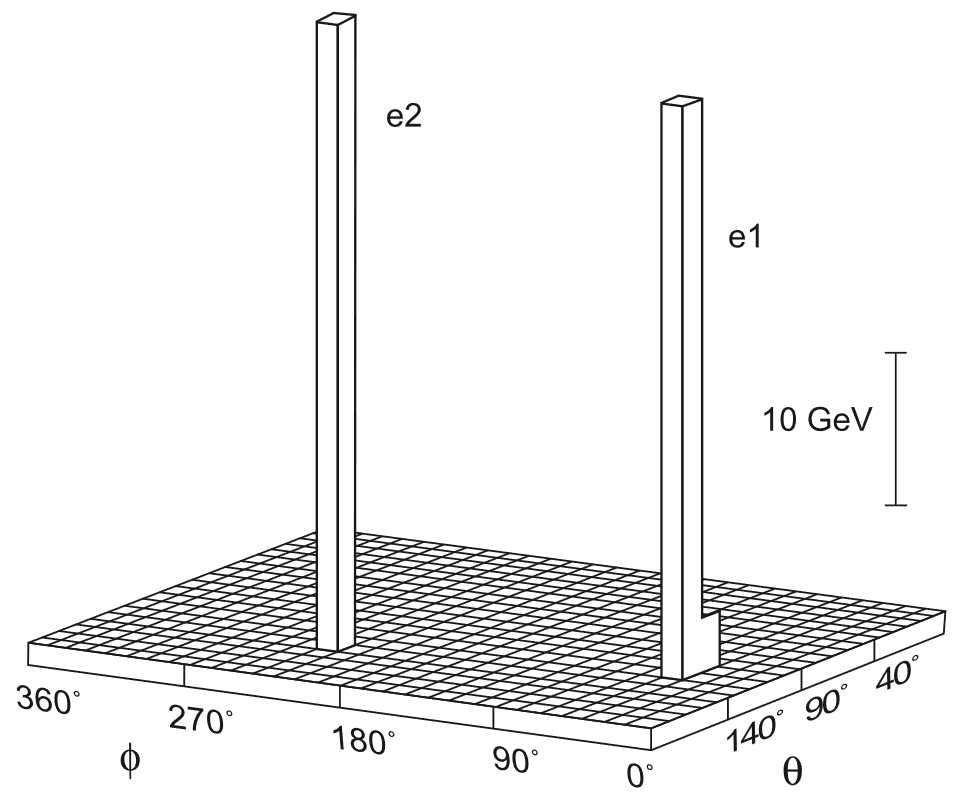
\includegraphics[width=6cm]{img/lego}
		\caption*{$q+\overline{q} \rightarrow Z^0 \rightarrow e^+ + e^-$ \cite{povh}}
	\end{figure}
\end{iframe}

\note[itemize] {
	\item Energie Summe $=$ Masse $Z^0$ (exakt?)
	\item Woher sicher, dass $Z^0$ Zerfall?
}

\subsection{Eigenschaften}
\begin{iframe}
	\framesubtitle{Experimentelle Bestimmung}
	\begin{itemize}
		\item Messung: %TODO Graphik!!
		\begin{itemize}
			\item $M_Z = \SI{91.188+-0.002}{GeV/c^2}$
			\item $\Gamma_Z = \SI{2.495+-0.002}{GeV}$
		\end{itemize}
		\pause
		\item Zerfall:
		\begin{align*}
			Z^0 \rightarrow & e^+ + e^- & \SI{3.363+-0.004}{\%} \\
			& \mu^+ + \mu^- & \SI{3.366+-0.007}{\%} \\
			& \tau^+ + \tau^- & \SI{3.370+-0.008}{\%} \\
			& \nu_{e,\mu,\tau}^+ + \overline{\nu}_{e,\mu,\tau} & \SI{20+-0.06}{\%} \\
			& \text{Hadronen} & \SI{69.91+-0.06}{\%} \\
		\end{align*}
	\end{itemize}
\note[item]{Über Wirkungsquerschnitt? src [PD12]}
\note[item]{}
\note[item]{Hadronen (idR. Anti+Quark) nicht unterscheidbar}
\note[item]{Anti+Neutrino schwer detektierbar => \% über $\Gamma_\text{tot}$}
\note[item]{totale Breite = alle Zerfälle Anti+Fermion???}
%\note[item]{$Z^0$ nicht nur ungeladenes $W$-Boson, da }
\end{iframe}

%TODO Neutrino generationen
